\documentclass{beamer}
\usetheme{COURS}
\usepackage{tcolorbox}
\usepackage{textpos}


\def\red{\color{red}}
\def\blue{\color{blue}}
\def\green{\color{green}}

\def\opstyle#1{\ensuremath{\operatorname{#1}}}


\title[Algorithmes combinatoires]%
{\bf Comptage et énumération de structures de données:
  \\ Algorithmes efficaces et implantations optimisées
}
\author{\textbf{\Large Florent Hivert}\\[5mm]
  Mél : \texttt{Florent.Hivert@lri.fr}\\
  Adresse universelle : \texttt{http://www.lri.fr/\~{ }hivert}
}
\date{}

\begin{document}
\newcommand{\Count}{\opstyle{count}}
\newcommand{\List}{\opstyle{list}}
\newcommand{\Iter}{\opstyle{iter}}
\newcommand{\Unrank}{\opstyle{unrank}}
\newcommand{\Rank}{\opstyle{rank}}
\newcommand{\First}{\opstyle{first}}
\newcommand{\Next}{\opstyle{next}}
\newcommand{\Random}{\opstyle{random}}
\newcommand{\Oh}{O}

%***********************************************************************
\frame{\titlepage}

%\begin{frame}
%   \slidepagestyle{empty}
%   \addtocounter{frame}{-1}
%   \maketitle
%\end{frame}

%***********************************************************************

\begin{frame}{Références}
  \begin{itemize}
  \item Frank Ruskey, \textit{Combinatorial Generation}
    \url{doi:10.1.1.93.5967}, 2003, non publié
    \bigskip

  \item A.~Nijenhuis and H.S.~Wilf, \textit{Combinatorial algorithms}, 2nd
    ed., Academic Press, 1978\\
    \url{http://www.math.upenn.edu/~wilf/website/CombinatorialAlgorithms.pdf}
    \bigskip

  \item The (Combinatorial) Object Server : \url{http://sue.csc.uvic.ca/~cos/}
    \bigskip

  \item The On-Line Encyclopedia of Integer Sequences \url{http://oeis.org}
  \end{itemize}
  \begin{textblock*}{100mm}(.75\textwidth,-8.2cm)
    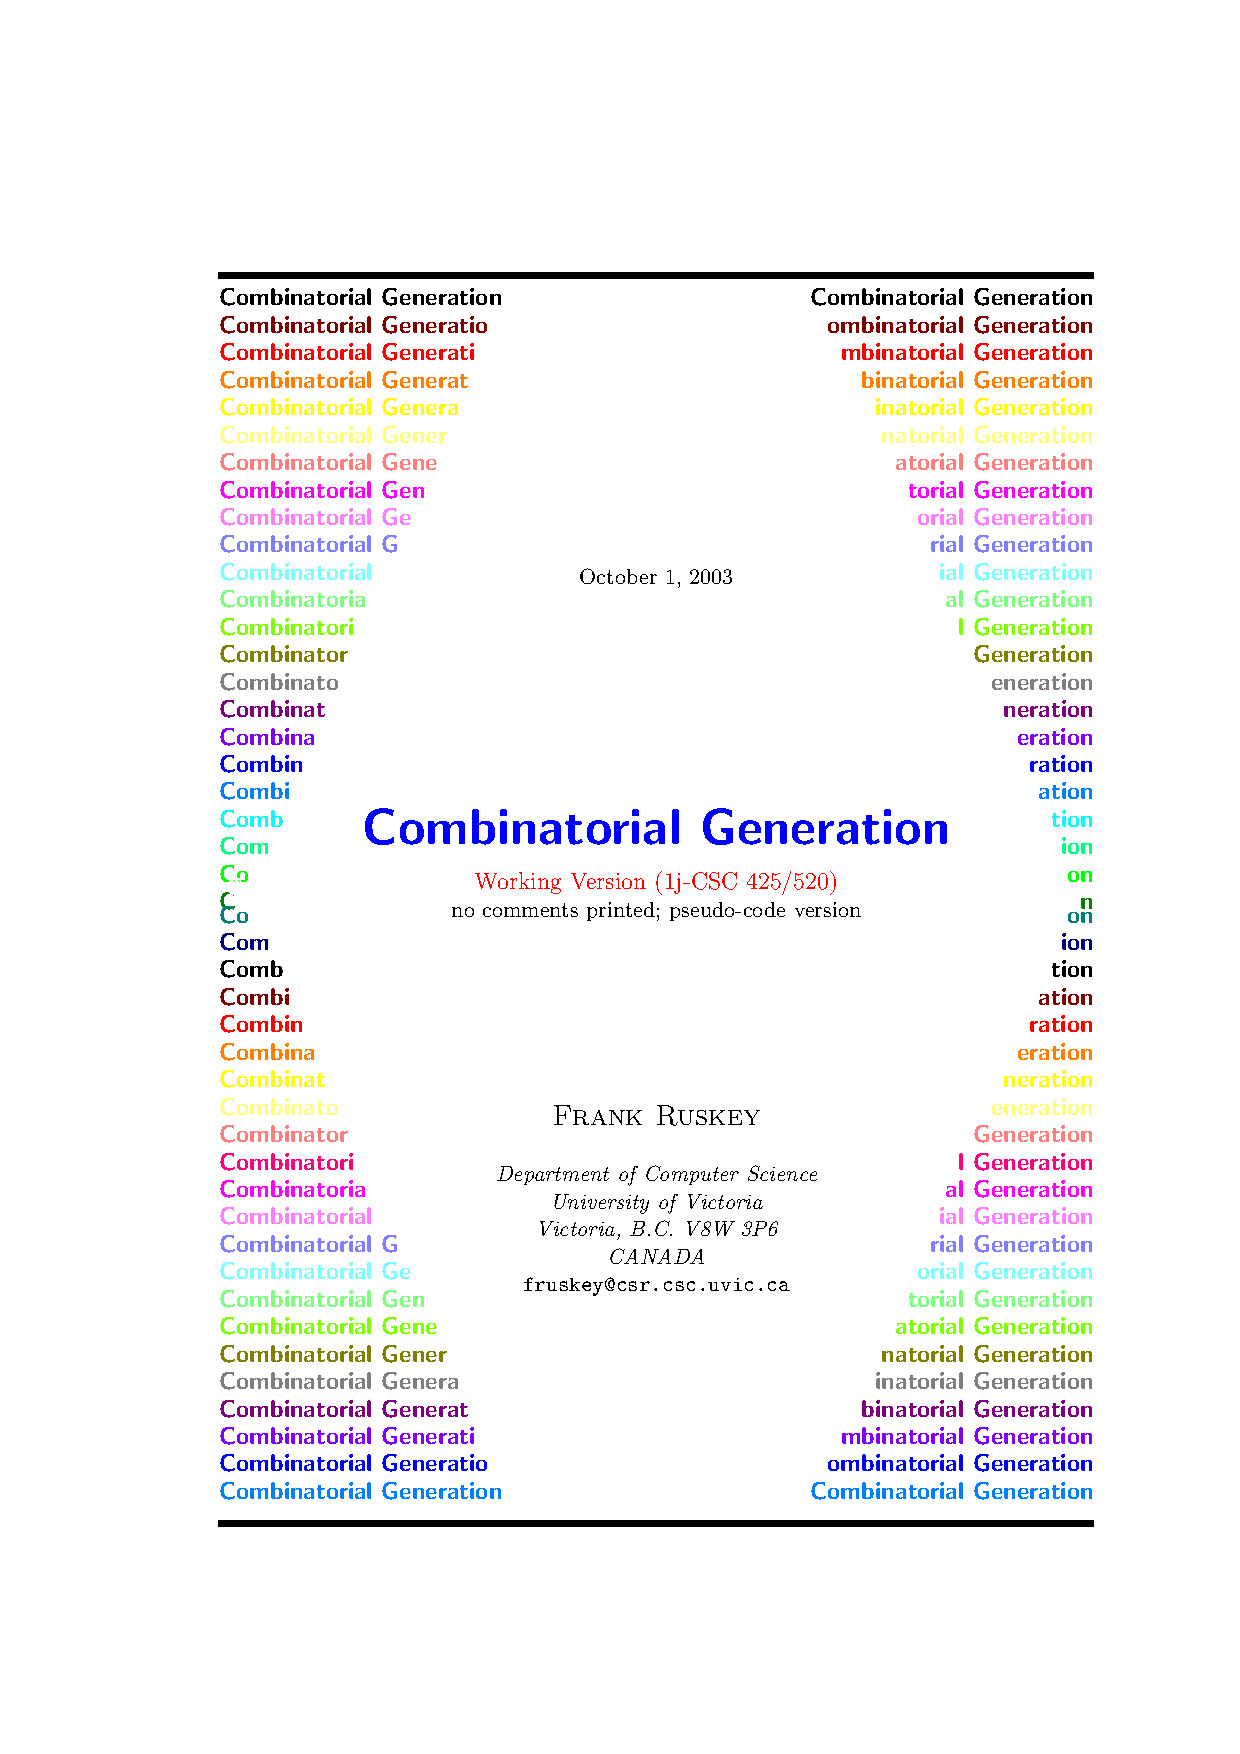
\includegraphics[width=2cm]{media/RuskeyCombGen-1.pdf}
  \end{textblock*}
\end{frame}

\begin{frame}{Algorithmes combinatoires}

  \begin{tcolorbox}
    \textbf{Manipulation d'ensembles finis}, mais souvent très grand...
  \end{tcolorbox}
  \bigskip

  \begin{tcolorbox}
    \textbf{Algorithmes et implantations efficaces} pour
    \begin{itemize}
    \item Compter, trouver la liste, itérer
    \medskip
    \item recherche d'un élément
    \medskip
    \item Tirage aléatoire équitable
    \end{itemize}
  \end{tcolorbox}
\end{frame}

\begin{frame}{Exemple d'ensemble finis...}

  Suite de $n$-bits:
  \begin{gather*}
    0\ 1 \\[4mm]
    00\ 01\ 10\ 11 \\[4mm]
    000\ 001\ 010\ 011\ 100\ 101\ 110\ 111 \\[4mm]
    0000\ 0001\ 0010\ 0011\ 0100\ 0101\ 0110\ 0111 \\
    1000\ 1001\ 1010\ 1011\ 1100\ 1101\ 1110\ 1111
  \end{gather*}
  Cardinal (nombre d'éléments) : \url{https://oeis.org/A000079}
  \[2^n : 1, 2, 4, 8, 16, 32, 64, 128, 256, 512, 1024, 2048, 4096 \dots\]
\end{frame}


\begin{frame}{Permutés de $[1,2,\dots,n]$}
  % print(r"\ ".join("".join(str(i) for i in p) for p in Permutations(1).list()))
  \begin{gather*}
    1 \\[4mm]
    12\ 21 \\[4mm]
    123\ 132\ 213\ 231\ 312\ 321 \\[4mm]
    1234\ 1243\ 1324\ 1342\ 1423\ 1432\ 2134\ 2143\ 2314\ 2341\ 2413\ 2431\\
    3124\ 3142\ 3214\ 3241\ 3412\ 3421\ 4123\ 4132\ 4213\ 4231\ 4312\ 4321
  \end{gather*}
  Cardinal (nombre d'éléments) : \url{https://oeis.org/A000142}
  \[n! : 1, 2, 6, 24, 120, 720, 5040, 40320, 362880, 3628800, 39916800 \dots\]
\end{frame}

\begin{frame}{Arbres binaires à $n$ noeuds}

  {\newcommand{\nodea}{\node[draw,circle] (a) {$$};}
  \newcommand{\nodeb}{\node[draw,circle] (b) {$$};}
  \newcommand{\nodec}{\node[draw,circle] (c) {$$};}
  \newcommand{\noded}{\node[draw,circle] (c) {$$};}
  \tiny
  \begin{gather*}
    \begin{tikzpicture}
      \matrix[column sep=.1cm, row sep=.1cm,ampersand replacement=\&]{
        \nodea \\
      };
    \end{tikzpicture}\\[4mm]
    %%%%%
    \begin{tikzpicture}
      \matrix[column sep=.1cm, row sep=.1cm,ampersand replacement=\&]{
        \& \nodea  \&         \\
        \&         \& \nodeb  \\
      };
      \path[ultra thick] (a) edge (b);
    \end{tikzpicture}
    \begin{tikzpicture}
      \matrix[column sep=.1cm, row sep=.1cm,ampersand replacement=\&]{
        \& \nodea  \&         \\
        \nodeb  \&         \&         \\
      };
      \path[ultra thick] (a) edge (b);
    \end{tikzpicture}\\[4mm]
    %%%
    \begin{tikzpicture}
      \matrix[column sep=.1cm, row sep=.1cm,ampersand replacement=\&]{
        \& \nodea  \&         \&         \&         \\
        \&         \&         \& \nodeb  \&         \\
        \&         \&         \&         \& \nodec  \\
      };
      \path[ultra thick] (b) edge (c)
      (a) edge (b);
    \end{tikzpicture}
    \begin{tikzpicture}
      \matrix[column sep=.1cm, row sep=.1cm,ampersand replacement=\&]{
        \& \nodea  \&         \&         \&         \\
        \&         \&         \& \nodeb  \&         \\
        \&         \& \nodec  \&         \&         \\
      };
      \path[ultra thick] (b) edge (c)
      (a) edge (b);
    \end{tikzpicture}
    \begin{tikzpicture}
      \matrix[column sep=.1cm, row sep=.1cm,ampersand replacement=\&]{
        \& \nodea  \&         \\
        \nodeb  \&         \& \nodec  \\
      };
      \path[ultra thick] (a) edge (b) edge (c);
    \end{tikzpicture}
    \begin{tikzpicture}
      \matrix[column sep=.1cm, row sep=.1cm,ampersand replacement=\&]{
        \&         \&         \& \nodea  \&         \\
        \& \nodeb  \&         \&         \&         \\
        \&         \& \nodec  \&         \&         \\
      };
      \path[ultra thick] (b) edge (c)
      (a) edge (b);
    \end{tikzpicture}
    \begin{tikzpicture}
      \matrix[column sep=.1cm, row sep=.1cm,ampersand replacement=\&]{
        \&         \&         \& \nodea  \&         \\
        \& \nodeb  \&         \&         \&         \\
        \nodec  \&         \&         \&         \&         \\
      };
      \path[ultra thick] (b) edge (c)
      (a) edge (b);
    \end{tikzpicture}
  \end{gather*}}
\end{frame}


\begin{frame}{Arbres binaires à $n$ noeuds}

  {\newcommand{\nodea}{\node[draw,circle] (a) {$$};}
  \newcommand{\nodeb}{\node[draw,circle] (b) {$$};}
  \newcommand{\nodec}{\node[draw,circle] (c) {$$};}
  \newcommand{\noded}{\node[draw,circle] (d) {$$};}
  \tiny
  \begin{gather*}
\begin{tikzpicture}
\matrix[column sep=.1cm, row sep=.1cm,ampersand replacement=\&]{
         \& \nodea  \&         \&         \&         \&         \&         \\
         \&         \&         \& \nodeb  \&         \&         \&         \\
         \&         \&         \&         \&         \& \nodec  \&         \\
         \&         \&         \&         \&         \&         \& \noded  \\
};
\path[ultra thick] (c) edge (d)
	(b) edge (c)
	(a) edge (b);
\end{tikzpicture}
\begin{tikzpicture}
\matrix[column sep=.1cm, row sep=.1cm,ampersand replacement=\&]{
         \& \nodea  \&         \&         \&         \&         \&         \\
         \&         \&         \& \nodeb  \&         \&         \&         \\
         \&         \&         \&         \&         \& \nodec  \&         \\
         \&         \&         \&         \& \noded  \&         \&         \\
};
\path[ultra thick] (c) edge (d)
	(b) edge (c)
	(a) edge (b);
\end{tikzpicture}
\begin{tikzpicture}
\matrix[column sep=.1cm, row sep=.1cm,ampersand replacement=\&]{
         \& \nodea  \&         \&         \&         \\
         \&         \&         \& \nodeb  \&         \\
         \&         \& \nodec  \&         \& \noded  \\
};
\path[ultra thick] (b) edge (c) edge (d)
	(a) edge (b);
\end{tikzpicture}
\begin{tikzpicture}
\matrix[column sep=.1cm, row sep=.1cm,ampersand replacement=\&]{
         \& \nodea  \&         \&         \&         \&         \&         \\
         \&         \&         \&         \&         \& \nodeb  \&         \\
         \&         \&         \& \nodec  \&         \&         \&         \\
         \&         \&         \&         \& \noded  \&         \&         \\
};
\path[ultra thick] (c) edge (d)
	(b) edge (c)
	(a) edge (b);
\end{tikzpicture}
\begin{tikzpicture}
\matrix[column sep=.1cm, row sep=.1cm,ampersand replacement=\&]{
         \& \nodea  \&         \&         \&         \&         \&         \\
         \&         \&         \&         \&         \& \nodeb  \&         \\
         \&         \&         \& \nodec  \&         \&         \&         \\
         \&         \& \noded  \&         \&         \&         \&         \\
};
\path[ultra thick] (c) edge (d)
	(b) edge (c)
	(a) edge (b);
\end{tikzpicture}\\
\begin{tikzpicture}
\matrix[column sep=.1cm, row sep=.1cm,ampersand replacement=\&]{
         \& \nodea  \&         \&         \&         \\
 \nodeb  \&         \&         \& \nodec  \&         \\
         \&         \&         \&         \& \noded  \\
};
\path[ultra thick] (c) edge (d)
	(a) edge (b) edge (c);
\end{tikzpicture}
\begin{tikzpicture}
\matrix[column sep=.1cm, row sep=.1cm,ampersand replacement=\&]{
         \& \nodea  \&         \&         \&         \\
 \nodeb  \&         \&         \& \nodec  \&         \\
         \&         \& \noded  \&         \&         \\
};
\path[ultra thick] (c) edge (d)
	(a) edge (b) edge (c);
\end{tikzpicture}
\begin{tikzpicture}
\matrix[column sep=.1cm, row sep=.1cm,ampersand replacement=\&]{
         \&         \&         \& \nodea  \&         \\
         \& \nodeb  \&         \&         \& \noded  \\
         \&         \& \nodec  \&         \&         \\
};
\path[ultra thick] (b) edge (c)
	(a) edge (b) edge (d);
\end{tikzpicture}
\begin{tikzpicture}
\matrix[column sep=.1cm, row sep=.1cm,ampersand replacement=\&]{
         \&         \&         \& \nodea  \&         \\
         \& \nodeb  \&         \&         \& \noded  \\
 \nodec  \&         \&         \&         \&         \\
};
\path[ultra thick] (b) edge (c)
	(a) edge (b) edge (d);
\end{tikzpicture}
\begin{tikzpicture}
\matrix[column sep=.1cm, row sep=.1cm,ampersand replacement=\&]{
         \&         \&         \&         \&         \& \nodea  \&         \\
         \& \nodeb  \&         \&         \&         \&         \&         \\
         \&         \&         \& \nodec  \&         \&         \&         \\
         \&         \&         \&         \& \noded  \&         \&         \\
};
\path[ultra thick] (c) edge (d)
	(b) edge (c)
	(a) edge (b);
\end{tikzpicture}\\
\begin{tikzpicture}
\matrix[column sep=.1cm, row sep=.1cm,ampersand replacement=\&]{
         \&         \&         \&         \&         \& \nodea  \&         \\
         \& \nodeb  \&         \&         \&         \&         \&         \\
         \&         \&         \& \nodec  \&         \&         \&         \\
         \&         \& \noded  \&         \&         \&         \&         \\
};
\path[ultra thick] (c) edge (d)
	(b) edge (c)
	(a) edge (b);
\end{tikzpicture}
\begin{tikzpicture}
\matrix[column sep=.1cm, row sep=.1cm,ampersand replacement=\&]{
         \&         \&         \& \nodea  \&         \\
         \& \nodeb  \&         \&         \&         \\
 \nodec  \&         \& \noded  \&         \&         \\
};
\path[ultra thick] (b) edge (c) edge (d)
	(a) edge (b);
\end{tikzpicture}
\begin{tikzpicture}
\matrix[column sep=.1cm, row sep=.1cm,ampersand replacement=\&]{
         \&         \&         \&         \&         \& \nodea  \&         \\
         \&         \&         \& \nodeb  \&         \&         \&         \\
         \& \nodec  \&         \&         \&         \&         \&         \\
         \&         \& \noded  \&         \&         \&         \&         \\
};
\path[ultra thick] (c) edge (d)
	(b) edge (c)
	(a) edge (b);
\end{tikzpicture}
\begin{tikzpicture}
\matrix[column sep=.1cm, row sep=.1cm,ampersand replacement=\&]{
         \&         \&         \&         \&         \& \nodea  \&         \\
         \&         \&         \& \nodeb  \&         \&         \&         \\
         \& \nodec  \&         \&         \&         \&         \&         \\
 \noded  \&         \&         \&         \&         \&         \&         \\
};
\path[ultra thick] (c) edge (d)
	(b) edge (c)
	(a) edge (b);
\end{tikzpicture}
\end{gather*}}
  Cardinal (nombre d'éléments) : \url{https://oeis.org/A000142}
  \[\operatorname{Cat}(n) : 1, 2, 5, 14, 42, 132, 429, 1430, 4862,
  16796, 58786, 208012 \dots\]
\end{frame}

\begin{frame}{Les graphes à $n$ noeuds:}
  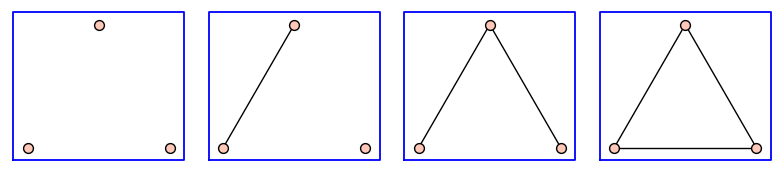
\includegraphics[width=5cm]{media/graphs-3.png}
\quad
  \raisebox{-1.3cm}{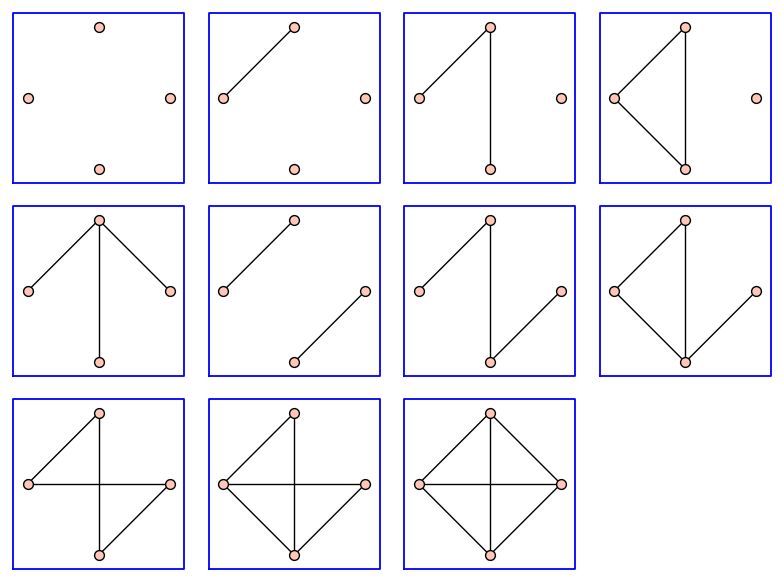
\includegraphics[width=5cm]{media/graphs-4.png}}
  \bigskip

  Cardinal (nombre d'éléments) : \url{https://oeis.org/A000088}
  \[\operatorname{Gr}(n) :
  1, 2, 4, 11, 34, 156, 1044, 12346, 274668, 12005168, 1018997864
  \dots\]
\end{frame}

\begin{frame}{Les graphes à $5$ noeuds:}

  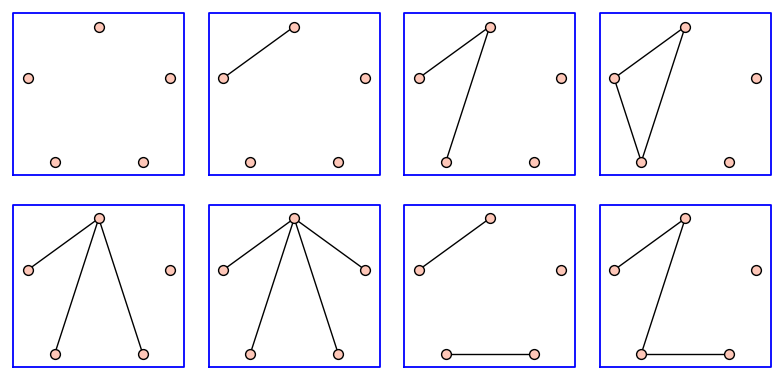
\includegraphics[width=5cm]{media/graphs-5-1.png}
  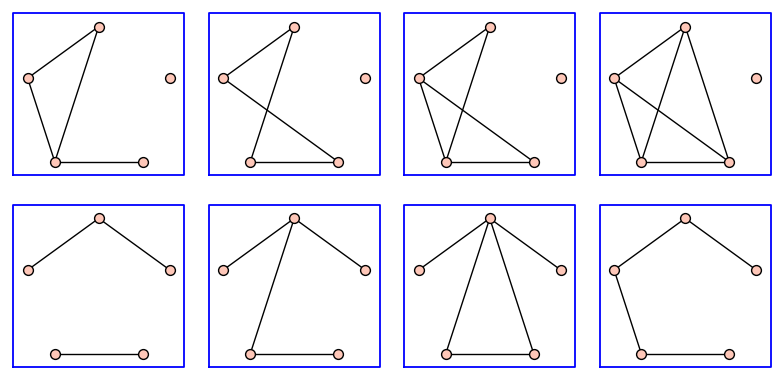
\includegraphics[width=5cm]{media/graphs-5-2.png}\\
  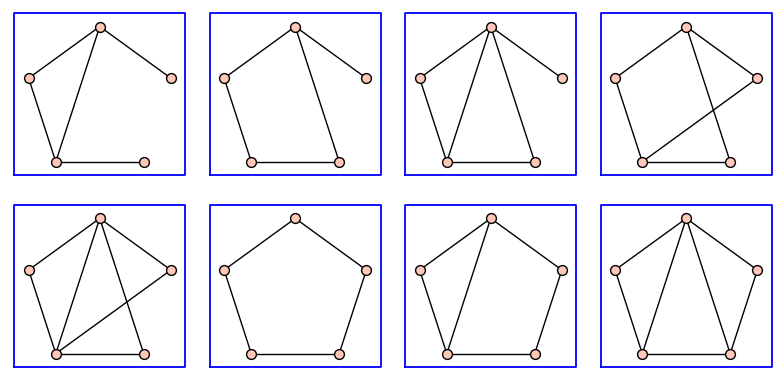
\includegraphics[width=5cm]{media/graphs-5-3.png}
  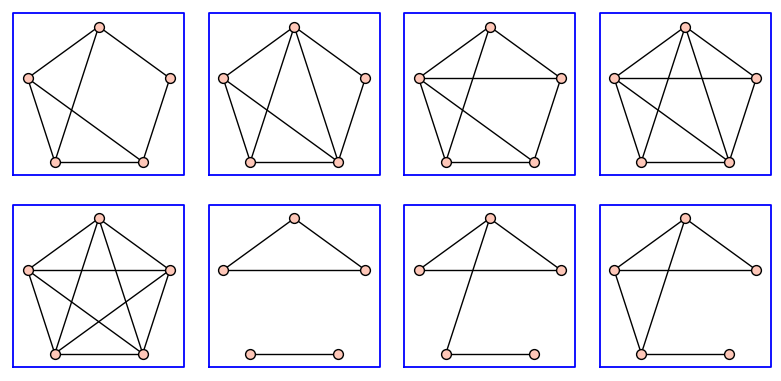
\includegraphics[width=5cm]{media/graphs-5-4.png}\\
  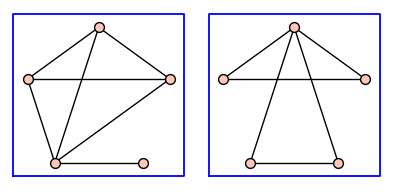
\includegraphics[width=2.5cm]{media/graphs-5-5.png}
\end{frame}

\begin{frame}{Manipulation d'ensembles finis:}

  ... mais souvent très grand ...
  \begin{itemize}
  \item suites de 64~bits: \texttt{0xce24762189cdef0d}
  \item permutés d'un tableaux: \texttt{[5,3,6,4,1,2]}
  \item arbres binaires à $7$~noeuds: \raisebox{-1cm}{\tiny\newcommand{\nodea}{\node[draw,circle] (a) {$$};}
 \newcommand{\nodeb}{\node[draw,circle] (b) {$$};}
 \newcommand{\nodec}{\node[draw,circle] (c) {$$};}
 \newcommand{\noded}{\node[draw,circle] (d) {$$};}
 \newcommand{\nodee}{\node[draw,circle] (e) {$$};}
 \newcommand{\nodef}{\node[draw,circle] (f) {$$};}
 \newcommand{\nodeg}{\node[draw,circle] (g) {$$};}\begin{tikzpicture}[auto]
\matrix[anchor=west,column sep=.05cm, row sep=.1cm,ampersand replacement=\&]{
         \&         \&         \&         \&         \& \nodea  \&         \&         \&         \\
         \&         \&         \& \nodeb  \&         \&         \&         \& \nodef  \&         \\
         \& \nodec  \&         \&         \&         \&         \& \nodeg  \&         \&         \\
 \noded  \&         \& \nodee  \&         \&         \&         \&         \&         \&         \\
};
\path[ultra thick] (c) edge (d) edge (e)
	(b) edge (c)
	(f) edge (g)
	(a) edge (b) edge (f);
\end{tikzpicture}}
  \item graphes à $8$-sommets:
    \raisebox{-1cm}{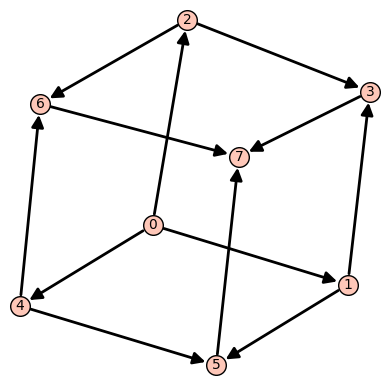
\includegraphics[width=2cm]{media/graphe.png}}
  \item document XML à $n$ balises
  \item programmes à $n$ caractères en C, chemin d'execution
  \end{itemize}
\end{frame}


\begin{frame}{Algorithmes combinatoires}

   Soit $S$ un ensemble \textbf{fini}.

   On souhaite écrire les algorithmes suivants: \bigskip

\begin{itemize}
\item \Count\ retourne le nombre d'éléments de $S$
\item \List\ retourne la liste des éléments de $S$
\item \Iter\ itère sur les éléments de $S$
\item \Unrank\ retourne le $i$-ème élement de la liste des éléments de $S$
\item \Rank\ étant donné $s\in S$ retourne sa position dans la liste
\item \First\ retourne le premier élément de la liste
\item \Next\ étant donné $s\in S$ retourne le suivant dans la liste
\item \Random\ retourne un $s\in S$ au hasard de manière équitable
\end{itemize}
\end{frame}

\begin{frame}{Applications}

  \begin{itemize}
  \item recherche de solution par la force brute
    \bigskip

  \item analyse d'algorithme, complexité
    \bigskip

  \item tests de programme, de système
    \bigskip

  \item recherche de failles, fuzzing
    \bigskip

  \item bio-informaique, chimie, physique statistique
  \end{itemize}
\end{frame}

\begin{frame}{Algorithme \List}

Soit $S$ l'ensemble des suites de 4~bits
\medskip

\begin{ALGO}[{{\red\List}}]
${\red\List(S)}$ retourne la liste des éléments de $S$
\end{ALGO}
\medskip\pause

Note: il faut fixer un ordre !
\medskip\pause

Par exemple pour l'ordre lexicographique:

\[ 0000,\ 0001,\ 0010,\ 0011,\ 0100,\ 0101,\ 0110,\ 0111 \]
\[ 1000,\ 1001,\ 1010,\ 1011,\ 1100,\ 1101,\ 1110,\ 1111 \]
\end{frame}

\begin{frame}{Algorithme \List}

  \begin{itemize}
  \item Version récursive:
    \[ B_n = 0\cdot B_{n-1}\ \cup\ 1\cdot B_{n-1}\]
    \pause\bigskip

  \item Version Itérative en utilisant la base 2.
  \end{itemize}
\end{frame}

\begin{frame}{Algorithme \Count}
\begin{ALGO}[{{\red\Count}}]
${\red\Count(S)}$ retourne le nombre d'éléments de $S$ (la cardinalité de
$S$).
\end{ALGO}
\bigskip\pause
Soit $S$ l'ensemble des suites de 4~bits
\medskip\pause
$$\Count(S) = 16$$
\end{frame}

\begin{frame}{Algorithme \Unrank}
\begin{ALGO}[{{\red\Unrank}}]
${\red\Unrank(S, i)}$ retourne le $i$-ème élement de la liste des éléments de
$S$ pour $0\leq i < \Count(S)$.
\end{ALGO}
\medskip\pause
Soit $S$ l'ensemble des suites de 4~bits dans l'ordre lexicographique
\[ 0000,\ 0001,\ 0010,\ 0011,\ 0100,\ 0101,\ 0110,\ 0111 \]
\[ 1000,\ 1001,\ 1010,\ 1011,\ 1100,\ 1101,\ 1110,\ 1111 \]
\medskip
Alors:
$$\Unrank(S, 11) = 1011$$
\end{frame}

\begin{frame}{Algorithme \Rank}
\begin{ALGO}[{{\red\Rank}}]
${\red\Rank(S, s)}$ retourne la position de $s \in S$ dans la liste
\end{ALGO}
\medskip\pause
Soit $S$ l'ensemble des suites de 4~bits dans l'ordre lexicographique
\[ 0000,\ 0001,\ 0010,\ 0011,\ 0100,\ 0101,\ 0110,\ 0111 \]
\[ 1000,\ 1001,\ 1010,\ 1011,\ 1100,\ 1101,\ 1110,\ 1111 \]
\medskip
Alors:
$$\Rank(S, 1011) = 11$$
\end{frame}

\begin{frame}{Algorithme \First}
\begin{ALGO}[{{\red\First}}]
${\red\First(S)}$ retourne le premier élément de la liste
\end{ALGO}
\medskip\pause
Soit $S$ l'ensemble des suites de 4~bits dans l'ordre lexicographique
\[ 0000,\ 0001,\ 0010,\ 0011,\ 0100,\ 0101,\ 0110,\ 0111 \]
\[ 1000,\ 1001,\ 1010,\ 1011,\ 1100,\ 1101,\ 1110,\ 1111 \]
\medskip
Alors:
$$\First(S) = 0000$$
\end{frame}

\begin{frame}{Algorithme \Next}
\begin{ALGO}[{{\red\Next}}]
${\red\Next(S, s)}$ retourne l'élément qui suit $s \in S$ dans la liste
\end{ALGO}
\medskip\pause
Soit $S$ l'ensemble des suites de 4~bits dans l'ordre lexicographique
\[ 0000,\ 0001,\ 0010,\ 0011,\ 0100,\ 0101,\ 0110,\ 0111 \]
\[ 1000,\ 1001,\ 1010,\ 1011,\ 1100,\ 1101,\ 1110,\ 1111 \]
\medskip\pause
Alors:
$$\Next(S, 1011) = 1100$$
\medskip\pause
et
$$\Next(S, 1111) = \text{Erreur ou Exception}$$
% TODO implem par defaut a partir de unrank
\end{frame}

\begin{frame}{Algorithme \Random}
\begin{ALGO}[{{\red\Random}}]
${\red\Random(S, s)}$ retourne un element de $s$ au hasard de manière équitable
\end{ALGO}
\medskip\pause
Soit $S$ l'ensemble des suites de 4~bits dans l'ordre lexicographique
\[ 0000,\ 0001,\ 0010,\ 0011,\ 0100,\ 0101,\ 0110,\ 0111 \]
\[ 1000,\ 1001,\ 1010,\ 1011,\ 1100,\ 1101,\ 1110,\ 1111 \]
\medskip\pause
Alors:
$$\Random(S)\text{ peut retourner }0011$$
\end{frame}


\begin{frame}{Algorithme \Iter}
\begin{ALGO}[{{\red\Iter}}]
${\red\Iter(S)}$ permet d'itérer sur les éléments de $S$
\end{ALGO}
\medskip\pause

Différents protocoles:
\begin{itemize}
\item objet avec une méthode \texttt{next} et exception (Python)
\item objet avec méthodes \texttt{next} et \texttt{hasNext} (Java)
\item objet avec passage au suivant \texttt{++}, déréférencement
  \texttt{*} et garde de fin (C++)
\item fonction de rappel (callback)
\item modèle producteur-consommateur (par ex. threads)
\end{itemize}
\end{frame}

\begin{frame}{Algorithme \Iter}
  \begin{NOTE}[\Iter\ vs. \List]
    Intérêts de \Iter\ par rapport à \List:
    \begin{itemize}
      \pause
    \item liste trop grande pour tenir en mémoire
      \pause
    \item algorithme en place, meilleur utilisation des caches de la mémoire
      \pause
    \item peut avoir une \textbf{complexité plus faible}
    \end{itemize}
  \end{NOTE}
\end{frame}

\begin{frame}{Notion de classe combinatoire}
  \begin{DEFN}[Classe combinatoire]
    On appelle \textbf{classe combinatoire} un ensemble $C$ dont les éléments
    $e$ ont une taille (nommée aussi degrée) noté $|e|$ et tels que l'ensemble
    $C_n$ des éléments de taille $n$ est fini:
    \[
    \Count(\{e\in C\ \mid\ |e| = n\}) < \infty
    \]
  \end{DEFN}
\end{frame}

\begin{frame}{Complexité de \List}
  Problème: liste des éléments de taille $n$.
  \pause
  \begin{PROP}
    La complexité de \List\ ne peut être meilleure que $\Oh(n\Count(C_n))$.
  \end{PROP}
\end{frame}

\begin{frame}{Complexité de \Iter}
  En revanche pour \Iter\ on peut obtenir
  \medskip

  \begin{DEFN}
    On dit qu'un algorithme est de complexité CAT (Constant Amortized Time)
    \textbf{temps constant amortis} si en moyenne chaque appel prend un temps
    constant.
  \end{DEFN}
  \bigskip\pause
  Ici, le nombre d'appel à la méthode \texttt{next} de l'itérateur est
  $\Count(C_n)$. Il faut donc que
  $$\frac{\text{Coût total des appels à
      \texttt{next}}}{\Count(C_n)}\in\Oh(1)$$
  \bigskip\pause
  Note: il n'y a pas de borne au coût d'un appel à la méthode \texttt{next}.
\end{frame}


\end{document}
